\documentclass[11pt]{article}

\usepackage[utf8]{inputenc} % Input encoding (allows æ, ø, å  fx)
\usepackage[T1]{fontenc} % Font encoding
\usepackage[backend=biber]{biblatex} % source tool
\usepackage[a4paper]{geometry} % Layout (margins, page size)
\usepackage{fourier} % Math font
\usepackage{inconsolata} % Monospace font
\usepackage{charter} % Font family
\usepackage[outputdir=build]{minted}
\usepackage[dvipsnames]{xcolor}
\usepackage[toc,page]{appendix}
\usepackage{graphicx}
\usepackage{pdfpages}
\usepackage{fancyhdr}
\usepackage{booktabs}
\usepackage{float}
\usepackage{enumitem}
\usepackage[hidelinks]{hyperref}
\usepackage{tocbasic}

\addbibresource{sources.bib}

\colorlet{LightGray}{Gray!5!}

\renewcommand*{\thesection}{Question~\arabic{section}:}
\renewcommand*{\thesubsection}{\arabic{section}.\alph{subsection}}
% \renewcommand*{\thesubsubsection}{\arabic{section}.\alph{subsection}.\roman{subsubsection}}
\renewcommand*{\thesubsubsection}{\texttt{\#}}

\newcommand*{\Appendixautorefname}{Appendix}

\DeclareTOCStyleEntry[dynnumwidth=true]{tocline}{section}

% \renewcommand{\baselinestretch}{1.2} % Line spacing
\setlength{\parindent}{0em} % Paragraph indent
\setlength{\parskip}{0.5em} % Paragraph vertical spacing

\newcommand{\code}[1]{
  % \tcbox[
  %   on line,
  %   boxsep=2pt,
  %   left=0pt, right=0pt, top=0pt, bottom=0pt,
  %   colback=LightGray,
  %   colframe=LightGray,
  % ]{{\mintinline{text}{#1}}}
  \mintinline{text}{#1}
}

\begin{document}
  \begin{titlepage}
    \newcommand{\HRule}{\rule{1.25\linewidth}{0.5mm}}
\center
\ \\[2cm]
\hbox{\makebox[1\textwidth][c]{\textsc{\Large Course: \textit{Operating Systems and C}}}}
\vspace{0.5cm}
\textsc{\large Course code: BSOPSYC1KU}
\\[0.2cm]
\textsc{\large Course manager: Willard Rafnsson}
\\[1cm]
\hbox{\makebox[1\textwidth][c]{\HRule}}
\vspace{0.4cm}
{ \huge \bfseries Operating Systems and C: Exam 2022}
\\[0.6cm]
\hbox{\makebox[1\textwidth][c]{\HRule}}
\vspace{0.9cm}
\textsc{\large IT University of Copenhagen}
\\[0.2cm]
\textsc{\large Bachelor in Software Development}
\\[1.5cm]
\begin{tabular}{ll}
\toprule
\textbf{Name} & \textbf{Email} \\
\midrule
Adrian Valdemar Borup & adbo@itu.dk \\
\bottomrule
\end{tabular}
\\[2cm]
{\large Dec 16 2022}
\\[2cm]
\vfill
  \end{titlepage}

  \pagestyle{fancy}
  \fancyhf{}
  \rhead{Adrian Borup (adbo)}
  \chead{Operating Systems and C exam}
  \lhead{Dec. 16 2022}
  \cfoot{\thepage}
  \newpage

  \setcounter{tocdepth}{2}
  \tableofcontents

  \newpage
  \section{Data Lab}
  \section{Data Lab}

\subsection{Implementation of \texttt{howManyBits(x)}}

The goal of this algorithm is to find the minimum number of bits required to represent the given 32-bit number using two's complement.

My implementation of \code{howManyBits(x)} has the following structure:

\begin{enumerate}
  \item Find the absolute value of \code{x}
  \item Find out how many bits are required to represent that value
  \item Add 1 to the result from step 2 to account for the sign bit
\end{enumerate}

Finding the absolute value of \code{x} lets us simplify the problem instead of handling positive and negative numbers separately. And once we've found the required number of bits to represent the 

Of these steps, step 2 is the crux. To solve this, my algorithm uses a binary search to find the most significant bit in the given number. The algorithm is as follows:

\begin{enumerate}
  \item See if there is a 1 in the first 16 bits of the number. If yes, we need at least 16 bits to represent the number. If no, we need at most 15 bits.
  \item Split the search space in half. If we found a 1, the new search space is the first half, and if not, it is the second half.
  \item Repeat steps 1 and 2 until 5 iterations have been performed.

    For the second iteration, we will be looking at 8 bits instead of 16. For the third iteration, we will be looking at 4 bits instead of 8, and so on.

    We can stop at 5 because the input is 32 bits long and $\log_2(32) = 5$.
\end{enumerate}

This may become more clear by reading the comments embedded in the code below and the example following that.

\subsubsection{Code and comments for \texttt{howManyBits(x)}}

Below is the full implementation of \code{howManyBits(x)} with comments that I handed in for the Data Lab assignment.

\bgroup
\small
\begin{minted}[bgcolor=LightGray]{c}
int howManyBits(int x) {
  // The general idea:
  // - Find the absolute value
  // - How many bits are required to represent that value?
  // - 1 more bit is needed for the sign

  // We find the absolute value of x. However, to avoid overflow issues with
  // -2147483648, we will have to subtract 1 from the absolute value if x is
  // negative - but the result we're looking for will be equally viable since
  // 0 is the most significant bit for positive two's complement numbers.
  int absMask = ~(1 & (x >> 31)) + 1;
  int abs = (~absMask & x) | (absMask & ~x);

  // We can now count how many bits we need to represent the unsigned number.
  // Due to the limited amount of operations we have at our disposal, we can't
  // search the 32 bits linearly - instead we use a binary search.
  //
  // The algorithm is as follows:
  //   1. Take a half-of-the-bits sized chunk out of the number - initially 16
  //      bits because the full number is 32 bits. That is, we will be looking
  //      at these bits first:
  //
  //          00000000 00000000 00000000 00000000
  //          ^^^^^^^^ ^^^^^^^^
  //
  //   2. Use !! to see if the bit chunk is nonzero
  int hasBits1 = !!(abs >> 16);
  //   3. Shift to the left by 4 (because 1 << 4 = 16, which is what we shifted
  //      right by). If there were any bits in the chunk, res1 now holds 16 as
  //      its value, but if no bits were present, its value is 0. If a bit was
  //      in the left half of the 32, we know we need at least 16 bits, so we
  //      hold onto this value for a bit (no pun intended).
  int res1 = hasBits1 << 4;
  //   4. Shift the number right by the amount of bits we know we need so far.
  //      By doing this, we perform the "binary search" aspect of the algorithm.
  //      If there was a bit in the left half, the next iteration will be
  //      looking at the first half of this left half - meaning these:
  //
  //          00000000 00000000 00000000 00000000
  //          ^^^^^^^^
  //
  //      That's thanks to us shifting the number right by 16 and the next
  //      iteration shifting right by 8. However, if no bit was in the left
  //      half, we shift right by 0, and the next iteration shifts right by 8.
  //      Therefore it will be looking in the first half of the right half:
  //
  //          00000000 00000000 00000000 00000000
  //                            ^^^^^^^^
  int abs1 = abs >> res1;
  //   5. Rinse and repeat with smaller and smaller halves until we've found how
  //      many bits we need in each.

  int hasBits2 = !!(abs1 >> 8);
  int res2 = hasBits2 << 3;
  int abs2 = abs1 >> res2;

  int hasBits3 = !!(abs2 >> 4);
  int res3 = hasBits3 << 2;
  int abs3 = abs2 >> res3;

  int hasBits4 = !!(abs3 >> 2);
  int res4 = hasBits4 << 1;
  int abs4 = abs3 >> res4;

  int hasBits5 = !!(abs4 >> 1);
  int res5 = hasBits5;
  int abs5 = abs4 >> res5;

  // 6. Add up all the different "I need at least X bits" results
  int unsignedBitsRequired = res1 + res2 + res3 + res4 + res5 + abs5;

  // And then we just need one more bit to represent signed numbers.
  return unsignedBitsRequired + 1;
}
\end{minted}
\egroup

\subsubsection{Example walkthrough of \texttt{howManyBits(x)}}

On the next page you can see a walkthrough of how the algorithm finds the answer given the input \code{4201337}. The left column will show all operations on and values of the variables at each step of the algorithm, and the right column will contain a description of the step. Grey bits indicate that we are no longer interested in those bits.

\newpage
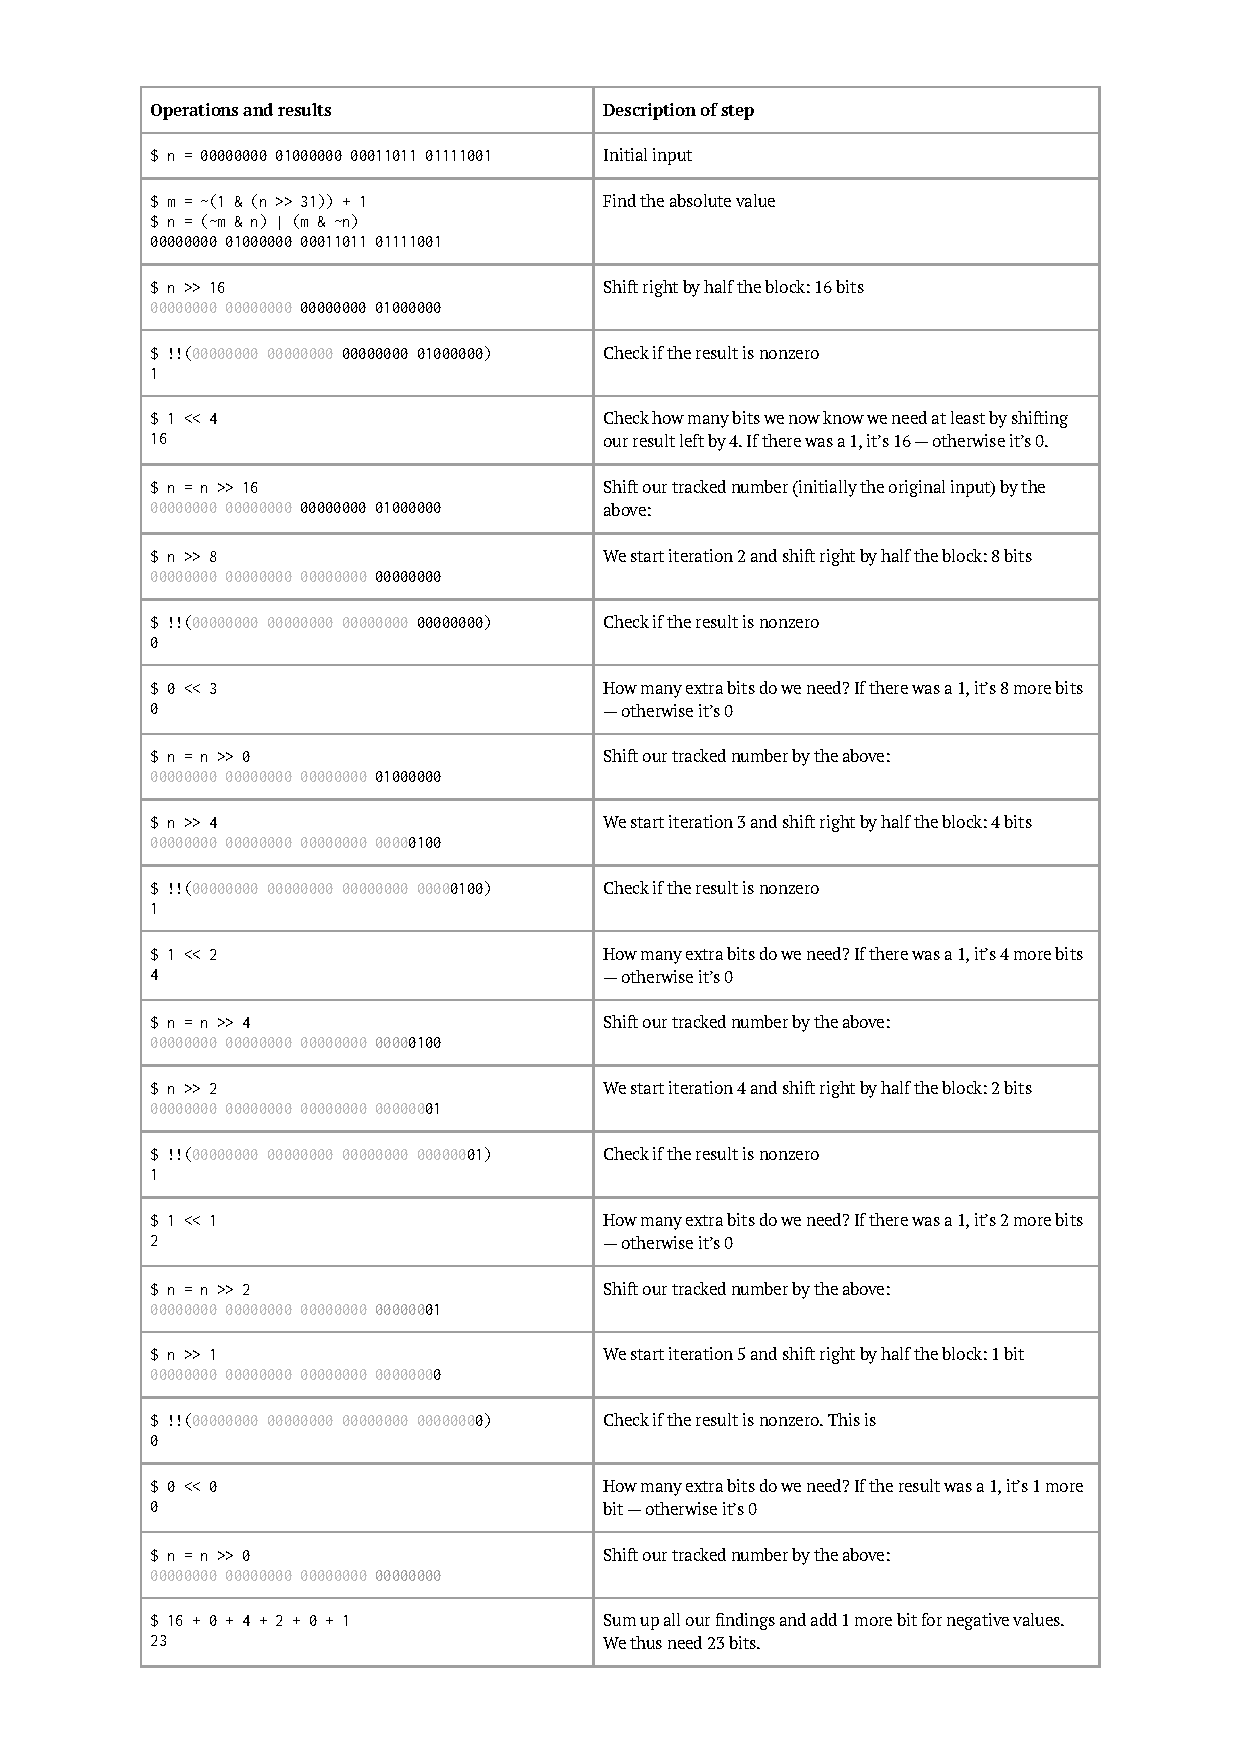
\includepdf[pages=-]{figures/howManyBits-example.pdf}
\newpage

  \subsection{Implementation of \texttt{tmin(void)}}

To determine the minimum number representable by two's complement, we have to be aware of how two's complement works. Two's complement reserves the most significant bit as a sign bit --- i.e. if the bit is set, the number is negative, and otherwise it's nonnegative.

One might implement signed integers intuitively in a way where positive and negative number pairs share all bits other than the sign bit (i.e. 3 and -3 would be represented as \code{011} and \code{111}, respectively). However, this is makes addition and overflow difficult to implement.

Two's complement is a way to make addition and subtraction easier to handle. To obtain that, the negative half of the numbers are represented in ``reverse'' (see \autoref{fig:twos-complement}). That is, for 4-bit integers, instead of having \code{1000} represent (negative) 0, we make it represent -8. Likewise, instead of having \code{1111} represent -7, we make it represent -1. This means that when you add 1 to the maximum number, you get the minimum number by nature of the representation.

\begin{figure}[H]
  \centering
  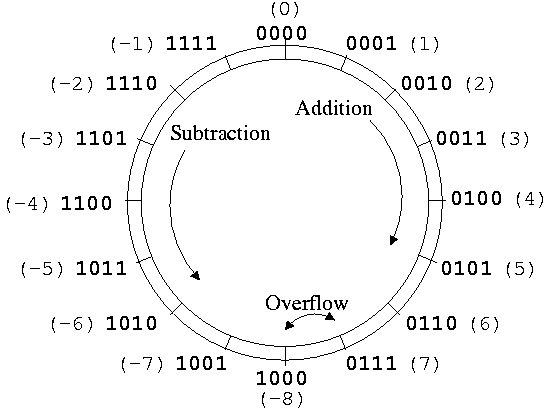
\includegraphics[width=0.7\textwidth]{figures/twos-complement.png}
  \caption[nothing]{An illustration of how integers are represented using two's complement~\cite{twoscomplement}.}
  \label{fig:twos-complement}
\end{figure}

With this in mind, we know that, by two's complement, the smallest number starts with a 1 followed by 0s only. Thus we can obtain the smallest number representable by two's complement by shifting a 1 to the most significant bit's position.

When you shift to the left with \code{<<}, all of the ``new'' bits on the right side are set to 0. For example \code{1011 << 2} becomes \code{1100} (assuming there is only space for 4 bits).

My complete implementation of \code{tmin(void)} is as follows:

\begin{minted}{c}
int tmin(void) {
  return 1 << 31;
}
\end{minted}

Because we are working with 32-bit numbers, shifting a 1 to the left by 31 bits will yield a single 1 in the most significant bit's position and nothing but 0s elsewhere. In decimal, this number is -2147483648.


  \section{Attack Lab}
  \subsection{The \texttt{c3} (\texttt{ret}) assembly instruction}

Assuming the x86 instruction set, \code{ret} does two things:

\begin{enumerate}
  \item Pops a memory address off the stack
  \item Jumps to that memory address
\end{enumerate}

What the CPU does in order to achieve the above is:

\begin{enumerate}
  \item Set the instruction pointer, which is stored in register \texttt{\%eip}~\cite{x86-control-flow}, to the value on top of the stack (at the address pointed to by register \texttt{\%rsp}).
  \item Decrease the stack pointer (in register \texttt{\%rsp}) with the address size (32 bits or 64 bits depending on architecture).
\end{enumerate}

I've illustrated this in an example on \autoref{fig:ret}:

\begin{figure}[H]
  \centering
  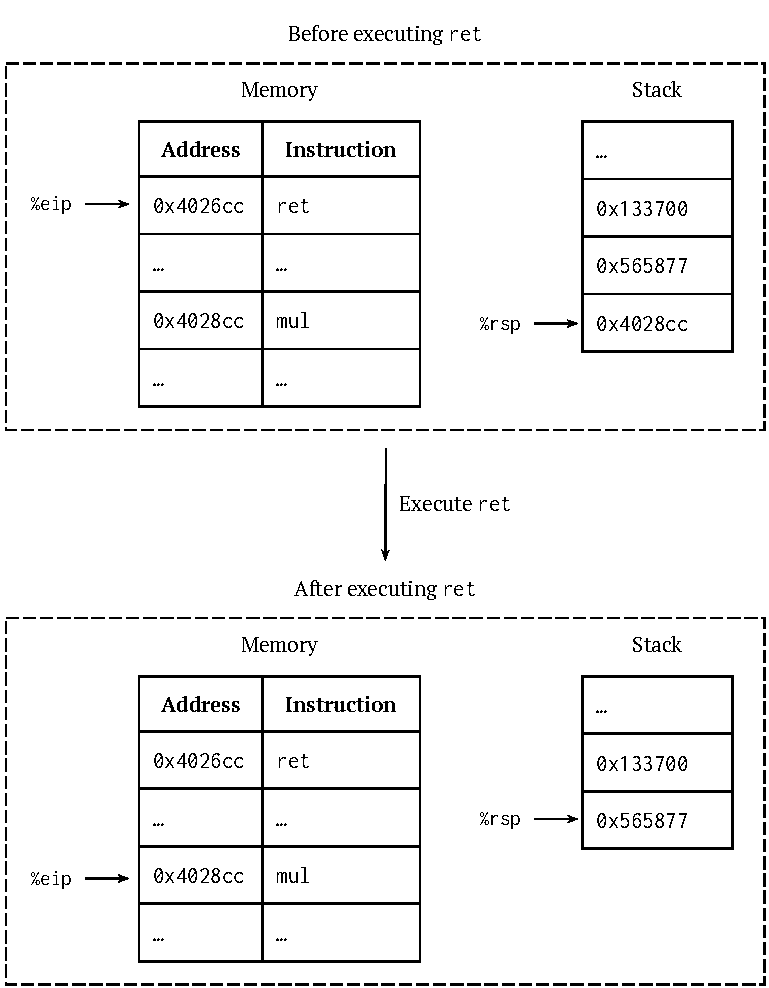
\includegraphics{figures/ret-example.pdf}
  \caption{An illustration of how the \code{ret} instruction manipulates registers in the CPU when executing the \code{ret} instruction. Before executing \code{ret}, the value \code{0x4028cc} is on top of the stack. After execution, the stack has been popped and the instruction pointer points to \code{0x4028cc}.}
  \label{fig:ret}
\end{figure}

  \subsection{Gadget farms}

\subsubsection{What is a gadget farm?}

``Gadgets'' are something used in return-oriented programming to execute code that already exists in a program rather than injecting new code.

An assembly program is represented by bytes. The CPU cannot tell the difference between a byte that was meant to be an instruction and a byte that was meant to be data. For example, the following is the object dump of my \code{getbuf} function from Attack Lab:

\begin{minted}{text}
000000000040267e <getbuf>:
  40267e:       f3 0f 1e fa             endbr64
  402682:       48 83 ec 28             sub    $0x28,%rsp
  402686:       48 89 e7                mov    %rsp,%rdi
  402689:       e8 b5 02 00 00          callq  402943 <Gets>
  40268e:       b8 01 00 00 00          mov    $0x1,%eax
  402693:       48 83 c4 28             add    $0x28,%rsp
  402697:       c3                      retq
\end{minted}

The intended instructions are listed line by line. However, if we have control over where the program will jump (for example by overwriting the base pointer), we can tell the CPU to execute instructions that were not ``intended'' to be there. For example, we can make the CPU execute the \code{ec} byte from the above assembly as an instruction by jumping to the address \code{0x402684}.

\begin{minted}{text}
  402682:       48 83 ec 28             sub    $0x28,%rsp
                      ^^
                     here
\end{minted}

In this case, it's just a useless instruction that ``inputs a byte from the I/O port in DX into AL''.\footnote{Source: \url{https://c9x.me/x86/html/file_module_x86_id_139.html}} With return-oriented programming, you attempt to find sequences of bytes in the assembly that execute instructions to your liking, which are then shortly followed by a \code{c3} byte. The \code{c3} byte, as described earlier, encodes the \code{ret} instruction. 

Recall that \code{ret} jumps to the address currently on top of the stack.
Therefore, if you have control of the stack, you can write addresses of multiple gadgets onto the stack that are then executed sequentially. When each gadget finishes, it \texttt{ret}s to the next address on the stack.

The gadget farm, in short, is a collection of all the gadgets we can find in the existing program code: addresses of groups of small, executable byte sequences that we can compose into larger and more useful gadgets.



  \section{Malloc Lab}
  \subsection{Implementation of \texttt{mm\_malloc}}

In order to make the concepts used in \code{mm_malloc} clearer, I will first explain how the dynamic memory allocator is laid out.

\subsubsection{Memory layout of my dynamic memory allocator}

My dynamic memory allocator uses the notion of blocks in the heap that are either allocated or free. To manage free blocks, I use an explicit free list, which will be described later.

Each block is 8-byte (double word) aligned and consists of a header, footer, and payload. Each block is laid out in memory as shown on \autoref{fig:block-layout} below.

\begin{figure}[H]
  \centering
  \hbox{\makebox[\textwidth][c]{
    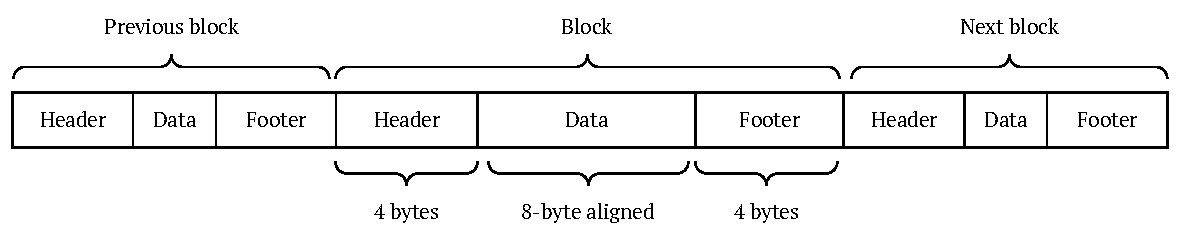
\includegraphics[scale=0.95]{figures/block-layout-example.pdf}
  }}
  \caption{The layout of blocks in memory for my dynamic memory allocator. ``Data'' is used synonymously with ``payload''.}
  \label{fig:block-layout}
\end{figure}

The header consists of the block's size and a flag that indicates if the block is allocated or free. This is all packed into a 32-bit integer. The size of the block is always a multiple of 8, meaning the least significant bit is always 0. Therefore, we can use this single bit to store the allocation flag.

The footer is a duplicate of the header, but it only exists for free blocks.

When we obtain a pointer to a block, the pointer points to the first byte of the payload, not the header.

For allocated blocks, the payload is where the user's data is written to. But for free blocks, because we are using an explicit free list, we use two words (8 bytes) in the payload to store two 4-byte pointers to the next and previous free blocks.

In order to avoid fragmentation, adjacent free blocks are joined every time a block is freed, or if the heap is extended. This means that the blocks in memory are not guaranteed to remain statically laid out --- their sizes can change.

\subsubsection{Components of my \code{mm_malloc} function}

The most important parts of my \code{mm_malloc} implementation (which will all be described in the next sections) are:

\begin{enumerate}
  \item \hyperref[sec:find-fit]{Finding a free block that's large enough}
  \item \hyperref[sec:extend-heap]{Optionally extending the heap}
  \item \hyperref[sec:manipulate-free-list]{Manipulating the free list}
  \item \hyperref[sec:place-block]{Placing the block}
\end{enumerate}

The code examples will use macros and constants for pointer arithmetic and utilities. The definition of these can be seen in \autoref{app:malloc-macros}.

\subsubsection{The explicit free list}
\label{sec:free-list}

It's possible to find a free block on the heap by iterating over all blocks. However, this takes $O(b)$ time (with $b$ being the amount of blocks). Instead, I've implemented an explicit free list, which uses the payload to store pointers to the next and previous free blocks. Using this is a doubly linked list, it's possible to iterate through only the free blocks on the heap, skipping all already-allocated blocks. The structure of free blocks in my implementation is illustrated on \autoref{fig:free-list-structure}.

\begin{figure}[H]
  \centering
  \hbox{\makebox[\textwidth][c]{
    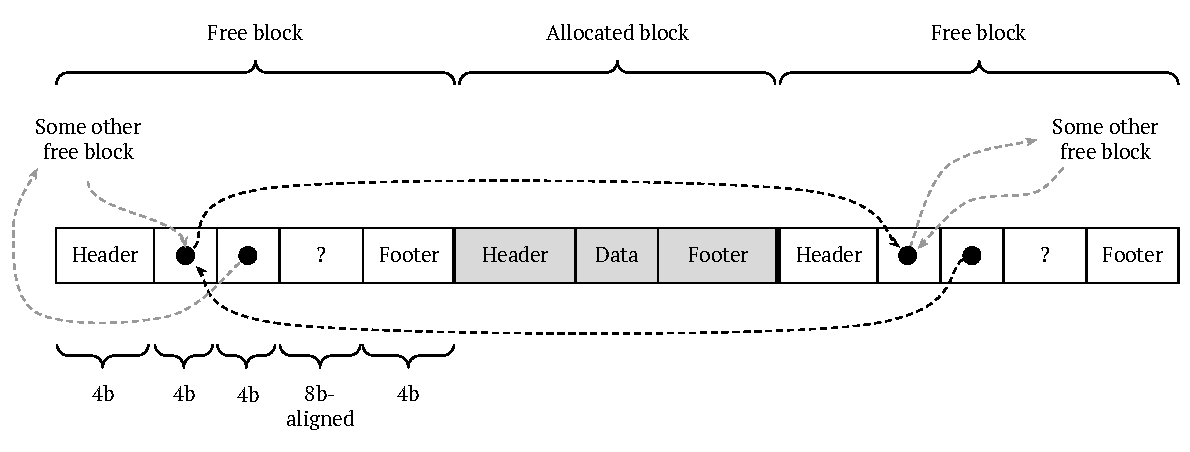
\includegraphics[scale=0.90]{figures/free-list-layout-example.pdf}
  }}
  \caption{An illustration of free blocks in my memory allocator. A block still has a header and footer, but it now also uses the first 8 bytes to store two 4-byte pointers to the next and previous free blocks, respectively. When there is no next or previous free block, the pointer is null. The \code{?} indicates that the rest of the data in a free block is just garbage.}
  \label{fig:free-list-structure}
\end{figure}

With this, it only takes $O(f)$ time (with $f$ being the amount of free blocks) in the worst case to find a free block large enough, if any such block exists.

\subsubsection{Finding a free block that's large enough}
\label{sec:find-fit}

Given the task to find a block of at least size \texttt{size}, it can be done rather straight forward using the explicit free list. Starting at the head of the linked list, we iterate over the entire free list and return a pointer to a free block if that block's size is at least \texttt{size}.

The code for my implementation is as follows:

\bgroup
\small
\begin{minted}[bgcolor=LightGray, linenos]{c}
static void *find_fit(size_t size)
{
    void *block_ptr = free_list;
    while (block_ptr != NULL)
    {
        if (get_size(get_header_ptr(block_ptr)) >= size)
            return block_ptr;

        block_ptr = get_next_free_block_ptr(block_ptr);
    }

    return NULL;
}
\end{minted}
\egroup

As can be seen, I did this using a first-fit search, rather than a best-fit search. This means I use the first block I find rather than the block on the free list where the needed space is as close as the block size as possible. This results in a faster lookup time, but it may cause more fragmentation.

\subsubsection{Optionally extending the heap}
\label{sec:extend-heap}

If no large enough free block can be found, it's necessary to extend the heap to accommodate the allocation request. To do that, the code below is used. An explanation will follow.

Disclaimer: the code for the \code{extend_heap} function has mostly been taken from the course book~\cite[p. 894]{computersystems} but has been modified slightly by me.

\bgroup
\small
\begin{minted}[bgcolor=LightGray, linenos]{c}
/* Increases the size of the heap with the given number of words */
static void *extend_heap(size_t words)
{
    char *bp;
    size_t size;

    /* Allocate an even number of words to maintain alignment */
    size = (words % 2) ? (words + 1) * WSIZE : words * WSIZE;
    if ((long)(bp = mem_sbrk(size)) == -1)
        return NULL;

    /* Initialize free block header/footer and the epilogue header */
    /* Free block header */
    set_val(get_header_ptr(bp), make_header(size, 0));
    /* Free block footer */
    set_val(get_footer_ptr(bp), make_header(size, 0));
    /* New epilogue header */
    set_val(get_header_ptr(get_next_block_ptr(bp)), make_header(0, 1)); 

    add_to_free_list(bp);

    /* Coalesce if the previous block was free */
    return coalesce(bp);
}
\end{minted}
\egroup

Line 8 ensures that the block size is satisfies our alignment.

On line 9, a call to \code{mem_sbrk} is made. This is synonymous to us using the \texttt{void *sbrk(intptr\_t incr)} function in C, which increases the program's data space by \code{incr} bytes \cite{sbrkmanpage}.

I didn't mention this earlier, but the heap is demarcated by two small blocks: the prologue and epilogue. These help the program stop searching at the correct spots. Lines 14-18 show how the empty epilogue block is moved from the current end of the heap to the new end of the heap.

On line 20, the newly allocated block is put onto the explicit free list.

To reduce external fragmentation when extending the heap and freeing blocks, adjacent free blocks are coalesced into a single free block. This is what happens on line 23. External fragmentation means that there is enough space in the heap to store a given size, but there is no single block large enough to hold it~\cite[p. 883]{computersystems}.

\subsubsection{Manipulating the free list}
\label{sec:manipulate-free-list}

When a block is allocated, it must be removed from the explicit free list. This works much like a doubly linked list, where addition and removal can be done in constant time. Adding a new free block is done by making it the new head of the list (\autoref{fig:free-list-add}), and removing a block is done by making its predecessor and successor point to each other (\autoref{fig:free-list-remove}).

\begin{figure}[H]
  \centering
  \hbox{\makebox[\textwidth][c]{
    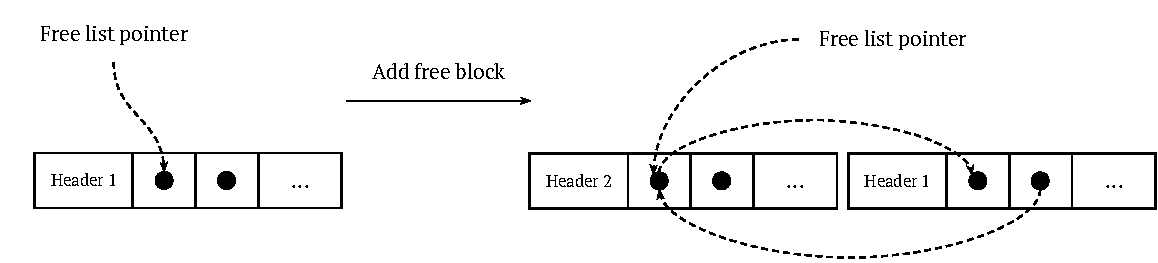
\includegraphics[scale=0.90]{figures/free-list-add-example.pdf}
  }}
  \caption{An illustration showing how to add a free block to the free list.}
  \label{fig:free-list-add}
\end{figure}

\begin{figure}[H]
  \centering
  \hbox{\makebox[\textwidth][c]{
    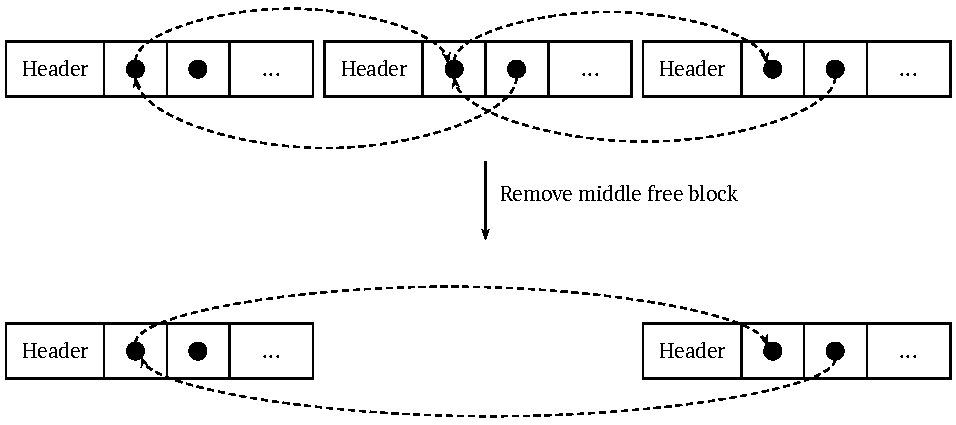
\includegraphics[scale=0.90]{figures/free-list-remove-example.pdf}
  }}
  \caption{An illustration showing how to remove a free block from the free list.}
  \label{fig:free-list-remove}
\end{figure}

The code to obtain that is as follows:

\bgroup
\small
\begin{minted}[bgcolor=LightGray, linenos]{c}
static void add_to_free_list(void *block_ptr)
{
    set_next_free_block_ptr(block_ptr, free_list);
    set_prev_free_block_ptr(free_list, block_ptr);
    set_prev_free_block_ptr(block_ptr, NULL);
    free_list = block_ptr;
}

static void remove_from_free_list(void *block_ptr)
{
    void *prev = get_prev_free_block_ptr(block_ptr);
    void *next = get_next_free_block_ptr(block_ptr);

    if (prev != NULL)
    {
        set_next_free_block_ptr(prev, next);
        set_prev_free_block_ptr(next, prev);
    }
    else
    {
        set_prev_free_block_ptr(next, NULL);
        free_list = next;
    }
}
\end{minted}
\egroup

When removing a block from the free list, there is one extra case to consider: if the block is currently the head of the free list, its successor should become the head of the free list instead. This is what happens on line 21-22.

\subsubsection{Placing the block}
\label{sec:place-block}

Once all the previously described work has been done, the block can be marked as allocated. Recall that it is the least significant bit of the header and footer that store this flag, therefore we simply need to set that bit to 1.

However, we can optimize the allocator with respect to memory utilization. Instead of simply marking the entire block as allocated, we can check if the block has space enough to be split into two blocks: one allocated block that uses just requested amount of space, and one free block with the spare space. This is especially useful because we use first-fit search, meaning the block we find may fit the requested size poorly.

\bgroup
\small
\begin{minted}[bgcolor=LightGray, linenos]{c}
static void place(void *ptr, size_t size)
{
    size_t cur_size = get_size(get_header_ptr(ptr));
    size_t remaining_size = cur_size - size;

    // There is space for another block, so we split
    if (remaining_size >= MIN_BLOCK_SIZE)
    {
        set_val(get_header_ptr(ptr), make_header(size, 1));
        set_val(get_footer_ptr(ptr), make_header(size, 1));

        void *next_block_ptr = get_next_block_ptr(ptr);
        set_val(get_header_ptr(next_block_ptr), make_header(remaining_size, 0));
        set_val(get_footer_ptr(next_block_ptr), make_header(remaining_size, 0));

        // Add the next block to the free list
        add_to_free_list(next_block_ptr);
    }
    // There is not space for another block, so we don't split
    else
    {
        set_val(get_header_ptr(ptr), make_header(cur_size, 1));
        set_val(get_footer_ptr(ptr), make_header(cur_size, 1));
    }
}
\end{minted}
\egroup

The first \texttt{if} block is executed when the found block is large enough to be split into two blocks. The first will be shrunk to the requested size and be marked as allocated. The second will be shrunk to the remaining size and added to the free list.

The \texttt{else} block will be executed if the block is not large enough, and it simply marks the block as allocated.

\subsubsection{The \code{mm_malloc} function}

Putting all the above together, I have implemented \code{mm_malloc} as follows:

\bgroup
\small
\begin{minted}[bgcolor=LightGray, linenos]{c}
void *mm_malloc(size_t size)
{
    // Ignore spurious requests
    if (size == 0)
        return NULL;

    // Adjust block size to include overhead and alignment reqs.
    // Size will always be at least 1 due to the check above
    size_t block_size = calc_block_size(size);

    // Search for a fitting block
    void *block_ptr = find_fit(block_size);

    if (block_ptr == NULL)
    {
        // No fit found. Get more memory.
        size_t extend_size = max(block_size, CHUNKSIZE);
        block_ptr = extend_heap(extend_size / WSIZE);
    }

    // The block is now allocated, so we remove it from the free list
    remove_from_free_list(block_ptr);

    // Write the header and footer to the heap (and split the block if there is
    // space left over)
    place(block_ptr, block_size);

    return block_ptr;
}
\end{minted}
\egroup

The procedure is simply:

\begin{enumerate}
  \item Adjust the requested size to 8 byte-alignment
  \item Find a free block that can fit the size
  \item If no block was found, extend the heap to obtain a free block large enough
  \item Remove the found block from the free list
  \item Mark the block as allocated and return a pointer to it
\end{enumerate}


  \subsection{Pointer arithmetic}

Pointer arithmetic is about performing addition and subtraction on pointers. However, the addition and subtraction behaviour differs depending on the types of the operands. In particular, when adding a number $n$ to a pointer type, the pointer is increased with $n \cdot t$, with $t$ being the size of the type being pointed to in bytes. For example, adding 1 to a \code{char *} pointer increases its value by 1, but adding 1 to an \code{int *} pointer increases its value by 4. The same applies for subtraction. I've created some examples of how adding to a pointer differs depending on the type being pointed to in \autoref{table:pointer-types}.

\begin{table}[H]
  \centering
  \begin{tabular}{lll}
    \toprule
    Type & Size in bytes & Pointer addition example \\ \midrule
    \code{char}      & 1 & \code{((char *) 0) + 1 = 0x1} \\
    \code{short}     & 2 & \code{((short *) 0) + 1 = 0x2} \\
    \code{int}       & 4 & \code{((int *) 0) + 1 = 0x4} \\
    \code{long long} & 8 & \code{((long long *) 0) + 1 = 0x8} \\
    \code{void}      & 1 & \code{((void *) 0) + 1 = 0x1} \\
    \code{char *}    & 4 & \code{((char **) 0) + 1 = 0x4} \\
    \bottomrule
  \end{tabular}
  \caption{Sizes of primitive types in C and examples of how adding 1 to each pointer type produces different results. The sizes were obtained in GDB with the \code{print sizeof(type)} command. The pointer addition was calculated with \code{print ((type *) 0) + 1}.}
  \label{table:pointer-types}
\end{table}

C disallows adding together two pointers because it conceptually doesn't make sense. For example, if you add \code{((char *) 0) + ((char *) 1)} to a C program, it will not compile. You can only add ``normal'' numbers to pointers.

However, C does allow subtraction of two pointers if the pointer types are the same size. Conceptually, the result of this corresponds to how many instances of that type can fit between the two pointees in memory. For example, take these two subtractions in GDB:

\begin{verbatim}
(gdb) print ((int *) 10) - ((unsigned int *) 1)
$1 = 2
(gdb) print ((char *) 10) - ((char *) 1)
$2 = 9
\end{verbatim}

Between memory address 10 and 1, you can fit 2 4-byte integers, but in the same memory range, you can fit 9 1-byte characters. Therefore the subtractions yield 2 and 9, respectively.

It's worth mentioning that indexing into an array with \code{arr[i]} is just a syntactic sugar for \code{*(arr + i)}. Arrays are just pointers, and the \texttt{i}th element is located at \code{arr} offset with \code{i} times the size of the array's element type (in bytes).

\subsubsection{How I use pointer arithmetic in \texttt{mm.c}}

Take this example:

\begin{minted}[breaklines]{c}
#define get_header_ptr(block_ptr) ((char *)(block_ptr)-WSIZE)
\end{minted}

Here, the given pointer \code{block_ptr} is cast to a \code{char *} so we that when we subtract \code{WSIZE}, we subtract exactly \code{WSIZE} bytes from the pointer. If we did not cast the pointer, the subtraction would depend on the pointer type given by the user. \code{WSIZE} is defined as the constant 4, so the following would have been equivalent:\\\code{(((int *)(block_ptr)) - 1)}.

Another example is how the footer pointer is computed:

\begin{minted}[breaklines]{c}
#define get_footer_ptr(block_ptr) ((char *)(block_ptr) + get_size(get_header_ptr(block_ptr)) - DSIZE)
\end{minted}

Similarly, the input pointer is cast to a \code{char *} for granular and more straight-forward pointer arithmetic. When we add \code{get_size(..)} to the block pointer, we add \code{get_size(..)} amount of bytes to the current block pointer --- i.e. we point to the next block. To point at the footer, \code{DSIZE} is subtracted, because subtracting 1 word yields the next block header location, and subtracting another word yields the current block's footer location.

Lastly, I use the below line of code to update a free block's ``previous block pointer'' field:

\begin{minted}[breaklines]{c}
set_val((char *)(block_ptr) + WSIZE, (unsigned int)next);
\end{minted}

The block pointer is cast to a \code{char *} so that when we add \code{WSIZE}, we add precisely 4 bytes. Equivalently, I could have written \code{(int *)(block_ptr) + 1}.

More usages of pointer arithmetic can be seen in \autoref{app:malloc-macros} on lines 23-33.


  \section{Topics from the class}
  \subsection{Exceptions: traps, faults, and aborts}

The very short version of the difference between traps, faults, and aborts is \cite[p. 762]{computersystems}:

\begin{description}[labelindent=1cm]
  \item[Traps] are expected by the programmer
  \item[Faults] are not expected (an error), but they can potentially be recovered from
  \item[Aborts] are not expected, and you cannot recover from them
\end{description}

All three are examples of synchronous exceptions, meaning they arise directly as the result of executing some instruction. What happens after the exception depends on the type of exception. After a trap handler finishes, control is returned to the next instruction in the program. When a fault occurs, control is transferred to a fault handler~\cite[765]{computersystems}. If the handler can successfully handle the error, the instruction that caused the fault is re-executed. Otherwise, the program is aborted. Aborts always cause the program to be aborted.

As an example, traps are used when making system calls. That is, request that the kernel perform some action and return to the running program afterwards. An example of a fault is a page fault, which happens when a physical page of memory is requested, but that page has not been mapped in virtual memory. This should be one that can be recovered from. Aborts can occur for \textit{many} reasons: division with 0, attempting to access memory outside the program, hardware errors, and many more. Aborts often surface as a ``general protection fault'' (typically presented as a ``segmentation fault'') \cite[p. 765]{computersystems}.

One extra note: an interrupt is another type of exception. It is an \textit{asynchronous} exception, caused by a signal being sent from an I/O device~\cite[p. 762]{computersystems}. For example, a network device may want to state that it has received a new connection request. Interrupts, like traps, also return control to the next instruction in the program~\cite[p. 763]{computersystems}.


  \printbibliography[heading=bibintoc]

  \newpage
  \begin{appendices}
    \section{Constants and macros used to implement \texttt{mm\_malloc}}
\label{app:malloc-macros}

Some of these are based on the course book \cite[p. 893]{computersystems}.

\bgroup
\small
\begin{minted}[bgcolor=LightGray, linenos, breaklines]{c}
/* single word (4) or double word (8) alignment */
#define ALIGNMENT 8
/* rounds up to the nearest multiple of ALIGNMENT */
#define align(size) (((size) + (ALIGNMENT - 1)) & ~0x7)

#define WSIZE 4             /* Word and header/footer size (bytes) */
#define DSIZE 8             /* Double word size (bytes) */
#define CHUNKSIZE (1 << 12) /* Extend heap by this amount (bytes) */

/* Pack a size and allocated bit into a word */
#define make_header(block_size, is_allocated) ((block_size) | (is_allocated))

/* Read and write a word at address p */
#define get_val(ptr) (*(unsigned int *)(ptr))
#define set_val(ptr, val) (*(unsigned int *)(ptr) = (val))

/* Read the size and allocated fields from pointer p */
#define get_size(ptr) (get_val(ptr) & ~0x7)
#define is_allocated(ptr) (get_val(ptr) & 0x1)
#define is_free(ptr) (!(is_allocated(ptr)))

/* Given block ptr bp, compute address of its header and footer. */
#define get_header_ptr(block_ptr) ((char *)(block_ptr)-WSIZE)
#define get_footer_ptr(block_ptr) ((char *)(block_ptr) + get_size(get_header_ptr(block_ptr)) - DSIZE)

/* Given block ptr bp, compute address of next and previous blocks */
#define get_next_block_ptr(block_ptr) ((char *)(block_ptr) + get_size(get_header_ptr(block_ptr)))
#define get_prev_block_ptr(block_ptr) ((char *)(block_ptr)-get_size(((char *)(block_ptr)-DSIZE)))

// Given a block pointer to a free block, get the free block it points to as the next one
#define get_next_free_block_ptr(block_ptr) ((void *)get_val(block_ptr))
// Given a block pointer to a free block, get the free block it points to as the previous one
#define get_prev_free_block_ptr(block_ptr) ((void *)get_val((char *)(block_ptr) + WSIZE))

/*
 * Given the size of the data, calculates how many bytes are needed to store the
 * block:
 *   - 1 word for header
 *   - 1 word for footer
 *   - 8-byte aligned data size
 */
#define calc_block_size(data_size) (WSIZE + WSIZE + align(data_size));

#define max(x, y) ((x) > (y) ? (x) : (y))
#define min(x, y) ((x) < (y) ? (x) : (y))

static int MIN_BLOCK_SIZE = calc_block_size(1);
\end{minted}
\egroup

  \end{appendices}
\end{document}
